\documentclass[12pt, A4]{article}
\usepackage[english,brazil]{babel}
\usepackage[utf8]{inputenc}
\usepackage[T1]{fontenc}
\usepackage{natbib}
\usepackage{url}
\usepackage{graphicx}
\usepackage{fancyhdr,multicol}
\usepackage{caption} 
\captionsetup{labelfont=bf}
\captionsetup[table]{skip=10pt}
\usepackage[paper=a4paper, textwidth=5.5in, top=1in, bottom=1.25in, headheight=.5in, headsep=0.5in, footskip=0.5in]{geometry}
\pdfpagewidth=\paperwidth
\pdfpageheight=\paperheight
\usepackage{longtable}
\usepackage{booktabs}
\usepackage{array}
\setlength{\parskip}{1ex plus 0.5ex minus 0.2ex} % espaco entre paragrafos e retira tabulacao no inicio
\newcommand{\R}{{\sf R}}
\newcommand{\code}[1]{\texttt{#1}}
\renewcommand{\footrulewidth}{0.5pt}
\begin{document}
%\maketitle
\pagestyle{fancyplain}
\lhead[] {\textsl{\footnotesize } \\ \textsl{\footnotesize Relatório Proc. FAPESP 2013/19250--7}}
\rhead[\fancyplain{}{\textsl{\thepage}}]%
      {\fancyplain{}{\textsl{\thepage}}}
\rfoot[]{\textsl{\footnotesize Laboratório de Ecologia Teórica -- IBUSP} \\
  \footnotesize \url{http://ecologia.ib.usp.br/let}}
\lfoot[]{\textsl{\footnotesize Jan/2015}}
\cfoot[]{}
\thispagestyle{empty}
%%%%%%%%%%%%%%%%%%%%%%%%%%%%%%%%%%%%%%%%%%%%%%%%%%%%%%%%%%%%%%%%%%%%%%%%%%%%%%%%%%%%%%%
%\vspace{-10in}
\begin{center}
  {\LARGE Relatório Científico de Andamento} 
\end{center}
\begin{description}
\item[Título do Projeto:] Ferramentas do Detetive Ecológico: uso e avaliação de modelos com detecção imperfeita
\item[Responsável:] Paulo Inácio de Knegt López de Prado
\item[Instituição-sede:] Instituto de Biociências, Universidade de São Paulo
\item[Equipe]{\bf:}
  \begin{itemize}
  \item Carlos Ernesto Candia-Gallardo, Pós-graduação em Ecologia IB--USP
  \item Gregório Menezes, consultor autônomo
  \item Gustavo Mattos Accacio, consultor autônomo
  \item Leonardo Liberali Wedekin, Pós-doutorado IB--USP
  \item Rodolpho Credo Rodrigues, Pós-graduação em Ecologia IB--USP
  \item Karlla Barbosa dos Santos, Bolsista TT-III FAPESP
  \item Melina de Souza Leite, Especialista em Laboratório, IB--USP
  \end{itemize}
\item[Processo:] 2013/19250-7 Auxílio Pesquisa - Regular 
\item[Vigência:] 01/02/2014 a 31/01/2016 
\item[Período deste relatório:] 01/02/2014 a 30/01/2015
\end{description}

\section{Resumo do projeto}

\subsection{Contexto e objetivo geral}
\label{sec:contexto}
O desenvolvimento e aplicação de teoria ecológica depende de estimativas
não-enviesadas e precisas da ocorrência, tamanho e taxas vitais de
populações naturais. Há uma percepção crescente de que
tais estimativas são fortemente afetadas por erros de observação, dos
quais as falsas ausências são o exemplo mais óbvio. Assim, o
pressuposto de detecção perfeita ou invariável de espécies e
indivíduos tem sido fortemente questionado, bem como os resultados que
dele derivam. Em resposta a esse problema desenvolveu-se um formalismo
de modelos estatísticos que separa dois níveis de
variação dos dados: a camada de observação e a camada do processo
biológico. Os  modelos hierárquicos com detecção
imperfeita são resultado desse formalismo. Têm implementações
computacionais acessíveis a ecólogos, e podem ser aplicadas em muito
mais casos do que têm sido. Por outro lado, essa nova abordagem
envolve procedimentos estatísticos mais complexos e um maior esforço
de amostragem. Assim, é necessário avaliar os ganhos efetivos dos
modelos com detecção imperfeita em diferentes tipos de pesquisas
ecológicas. O objetivo desta proposta é usar estimativas de
ocorrência, abundância e taxas vitais de espécies obtidos com modelos
de detecção imperfeita em três estudos de casos que juntos abrangem
testes sobre estrutura e dinâmicas de populações e comunidades, em
aspectos teóricos e aplicados. Além da importância teórica e aplicada
dos estudos de caso em si, vamos avaliar a sensibilidade dos
resultados e conclusões à adoção da abordagem de modelos com detecção
imperfeita.

\subsection{Objetivos específicos}
\label{sec:especificos}
\begin{enumerate}
\item Testar se mudanças temporais na abundância relativa e
  diversidade de borboletas nectarívoras de subosque  
  são condizentes com previsões da Teoria Neutra ou com
  previsões de modelos baseados em nicho. 
\item Investigar se a correlações entre a diversidade de estratos da
  vegetação e diversidade de aves de cerrado é explicada pelos padrões
  de uso e sobreposição de uso desses estratos pelas aves.
\item Investigar os efeitos de flutuações climáticas a nível global na
  dinâmica populacional das baleias-jubarte que usam as águas
  brasileiras como área de reprodução.
\item Avaliar o impacto do uso das estimativas com detecção imperfeita
  sobre as conclusões obtidas no três estudos de caso acima.
\end{enumerate}

\section{Resultados do período}

\subsection{Borboletas: dinâmica de comunidades e neutralidade} %Kiwi
\label{sec:dinamica-temporal-borb} 

Até o momento realizamos amostragens regulares de
captura-marcação-recaptura de borboletas Ithomiini (Nymphalidae,
Danainae, Fig.~\ref{fig:2.1.1}) 
em duas áreas da Cidade Universitária em São Paulo (USP). Na
primeira, o Parque Esporte Para Todos (PEPT), as amostragens
iniciaram-se em abril de 2013 e até dezembro de 2014 haviam sido
realizadas 24 campanhas. A frequência de coletas foi
quinzenal de abril a julho de 2013 e mensal após este
período. As coletas da segunda área - Reserva
Florestal da Cidade Universitária - iniciaram-se em fevereiro de 2014
e até dezembro de 2014 haviam sido realizadas 11 campanhas. Prosseguiremos
os censos em ambas as áreas pelo menos até dezembro de 2015,
com frequência mensal. Aqui serão reportados os dados obtidos até
dezembro de 2014, porém algumas análises usam dados apenas até outubro de 2014.
Capturamos 7.758 indivíduos de Ithomiini (mais 2784 recapturas) : 
5.939 no PEPT (mais 2.309) recapturas) e 1.864 na Reserva Florestal (mais 520 recapturas). 
Ao todo registramos 22 espécies divididas em nove subtribos, 
representando sete anéis miméticos diferentes (Tab.~\ref{tab:borb1} e Fig.~\ref{fig:2.1.2}).

Como observado em qualquer comunidade biológica, o número de
indivíduos capturados em ambas as áreas não foi homogeneamente
distribuído entre as espécies. A maioria dos indivíduos pertenceu a
poucas espécies, sendo que das 22 espécies registradas apenas oito
tiveram número de capturas
suficiente para que parâmetros demográficos possam ser calculados
(Fig.~\ref{fig:2.1.2}). 


\begin{table}
  \centering
  \caption{Número de capturas (Cap) e recapturas (Rec) de indivíduos 
    de borboletas da tribo
    Ithomiini (Lepidoptera, Nymphalydae, Danainae) no Parque
    Esporte Para Todos (PEPT) e na Reserva Florestal (RF), ambas no campus da
    USP. Taxonomia e nomenclatura seguem proposta de \citet{Brower_2014}. 
    Anel mimético definido de acordo com \citet{Willmott_2004}}
  \begin{tabular}{llrrrr}
    \toprule
    & &\multicolumn{2}{c}{\textbf{PEPT}} & \multicolumn{2}{c}{\textbf{RF}} \\
    \textbf{Taxon} & \textbf{Anel} & \textbf{Cap} & \textbf{Rec} & \textbf{Cap} & \textbf{Rec}\\
    \midrule
    \emph{Aeria olena} & Agna & 5 & 3 & 0 & 0\\
    \emph{Dircenna dero} & Themisto & 41 & 3 & 19 & 0\\
    \emph{Episcada carcinia} & Aquata & 4 & 0 & 7 & 0\\
    \emph{Episcada clausina} & Aquata & 10 & 1 & 9 & 0\\
    \emph{Episcada hymenaea} & Hymenaea & 45 & 5 & 32 & 0\\
    \emph{Episcada philoclea} & Philoclea & 0 & 0 & 1 & 0\\
    \emph{Epityches eupompe} & Philoclea & 285 & 63 & 74 & 5\\
    \emph{Heterosais edessa} & Aquata & 10 & 0 & 0 & 0\\
    \emph{Hypoleria lavinia} & Aquata & 212 & 65 & 193 & 49\\
    \emph{Hypothyris euclea laphria} & Ethra & 448 & 189 & 224 & 117\\
    \emph{Hypothyris ninonia daeta} & Lysimnia & 1539 & 1164 & 359 & 204\\
    \emph{Ithomia agnosia zikani} & Aquata & 1999 & 435 & 546 & 65\\
    \emph{Ithomia drymo} & Aquata & 16 & 2 & 9 & 1\\
    \emph{Mcclungia cymo salonina} & Philoclea & 248 & 48 & 58 & 4\\
    \emph{Mechanitis lysimnia} & Lysimnia & 230 & 82 & 87 & 33\\
    \emph{Mechanitis polymnia} & Ethra & 771 & 238 & 182 & 36\\
    \emph{Melinaea ludovica paraiya} & Ethra & 1 & 0 & 0 & 0\\
    \emph{Methona themisto} & Themisto & 10 & 0 & 1 & 0\\
    \emph{Oleria aquata} & Aquata & 8 & 1 & 11 & 5\\
    \emph{Placidina euryanassa} & Lysimnia & 2 & 0 & 4 & 0\\
    \emph{Pseudoscada acilla} & Aquata & 29 & 6 & 18 & 0\\
    \emph{Pseudoscada erruca} & Aquata & 21 & 3 & 10 & 1\\
    \textbf{TOTAL} & & \textbf{5934} & \textbf{2308} & \textbf{1844} & \textbf{520}\\
    \bottomrule
  \end{tabular} 
  \label{tab:borb1}
\end{table}

\begin{figure}
  \centering
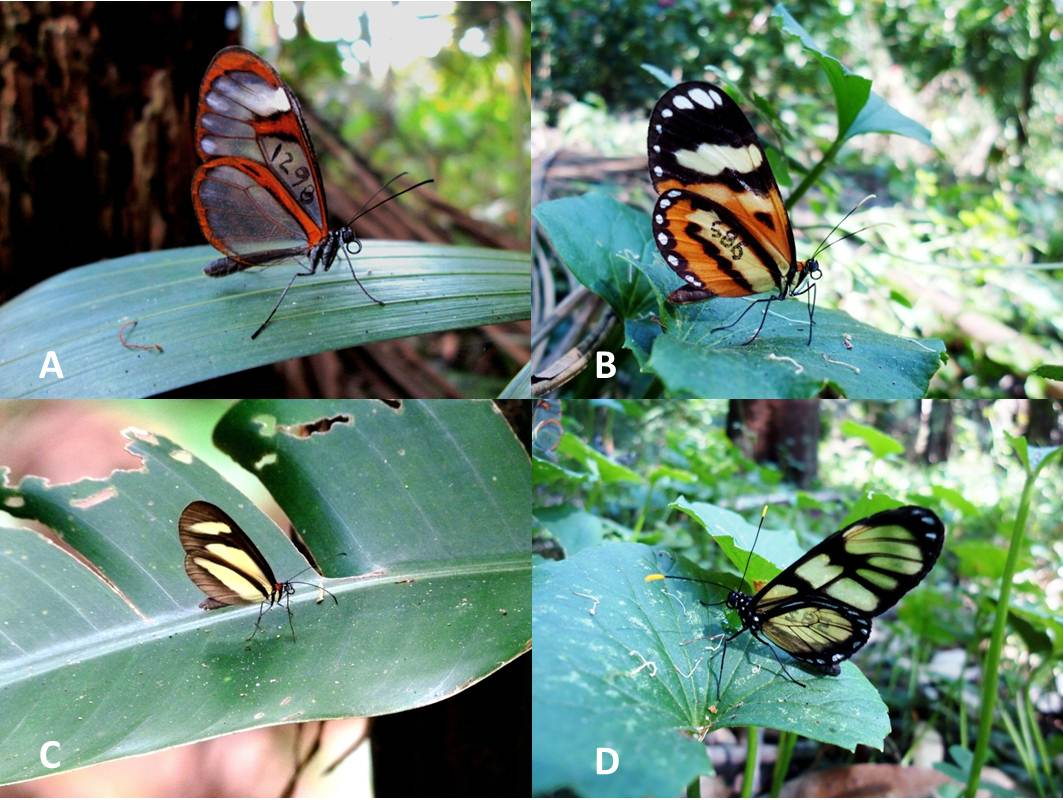
\includegraphics[width=0.75\textwidth]{figures/Imagem11/Imagem11}
  \caption{Espécies de Ithomiini pertencentes a diferentes anéis miméticos registradas ao longo deste estudo: A - \textit{Hypoleria lavinia} ; B - \textit{Hypothyris ninonia}; C - \textit{Aeria olena}; e D - \textit{Dircenna dero}. Note as marcações nos indivíduos A, B e D, que são números escritos com caneta permamente nas asas.}
\label{fig:2.1.1} 
\end{figure}

\begin{figure}
  \centering
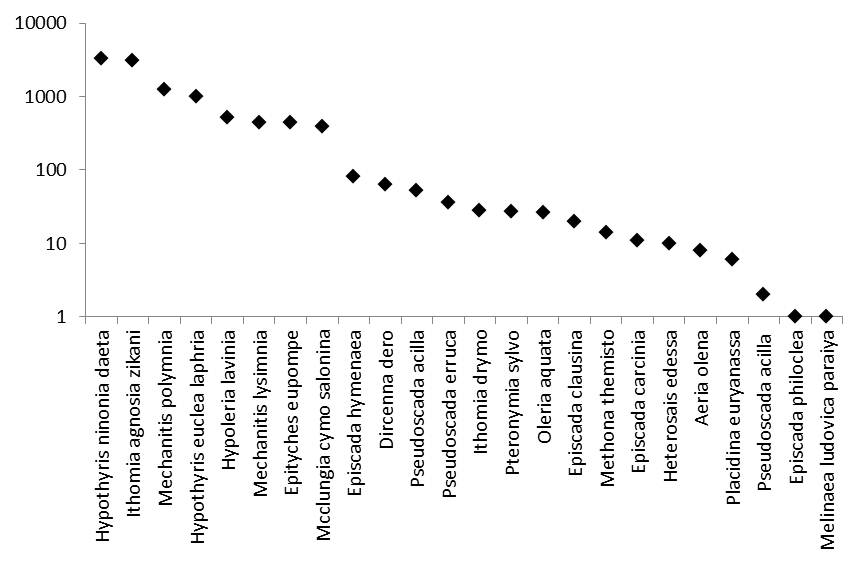
\includegraphics[width=\textwidth]{figures/Imagem2/Imagem1.jpg}
  \caption{Distribuição de abundância de espécies (DAE) de Ithomiini (Nymphalidade, Danainae) 
    capturadas no Parque Esporte Para Todos (PEPT) e na Reserva Florestal da Cidade Universitária da USP. 
    Dados acumulados de abril/13 a dezembro/14.}
\label{fig:2.1.2} 
\end{figure}


\subsection{Dinâmica temporal}
\label{sec:din-temp-borb}
A distribuição temporal das capturas de indivíduos de Ithomiini não
foi homogênea entre os meses. Foram observadas grandes concentrações
de indivíduos nos meses mais secos (maio a agosto) e números de
indivíduos consideravelmente mais baixos nos meses chuvosos
(Fig.~\ref{fig:2.1.3}). Estas agregações sazonais de Ithomiini –
sempre durante a estação menos chuvosa - já foram observadas em
regiões onde ocorre uma estação relativamente mais seca ao longo do
ano, como em Campinas \citep{brown2002} e Caldas Novas
\citep{Pinheiro_2008}.

As abundâncias – representadas pelo número bruto de capturas - das
espécies de Ithomiini capturadas no Parque Esporte Para Todos (PEPT)
variaram consideravelmente entre os meses. Espécies inicialmente raras
(ou ausentes) aumentaram em número em meses posteriores e vice-versa,
evidenciando a existência de rotatividade (\emph{turnover}) considerável nas
Distribuições de Abundâncias de Espécies (DAE) obtidas em cada mês
(Fig.~\ref{fig:2.1.4}).

Para mensurar a rotatividade na composição e
abundância da comunidade de Ithomiini do Parque Esporte Para Todos
calculamos a similaridade (Bray-Curtis) das amostras de cada mês em
relação ao centroide da comunidade, o qual foi obtido com a
média do número de indivíduos de cada espécie capturados em todos os
meses de amostragem. Os resultados revelam uma tendência de queda na
similaridade da comunidade em relação ao seu centroide na estação
chuvosa e um posterior aumento na estação seca (Fig.~\ref{fig:2.1.5}).

A curva espécies tempo baseada em indivíduos obtida no Parque Esporte
para Todos de abril/13 a out/14 está representada na
figura~\ref{fig:2.1.6}. É possível notar uma tendência à estabilização
da curva indicando que as espécies mais comuns da comunidade foram
registradas e que novas espécies que eventualmente podem ser
capturadas devem ser representadas por espécies ocasionais.

Percebemos que a dinâmica caracterizada pelo procedimento de marcação e recaptura
é a de formação e dissolução do bolsão na estação seca. 
Nesta fase é razoável a premissa de fechamento da população nas instâncias primárias
de amostragem (manhãs e tardes de dois dias consecutivos). Além disso, é na fase de bolsões
que é possível obter capturas e recapturas em número suficiente para estimar os parâmetros
da dinâmica (taxas de entrada e saída de indivíduos). Portanto, concentraremos 
o teste de neutralidade à dinâmica dos bolsões. 
Durante este processo, há um considerável \emph{turnover} temporal de dominância.
Nossa principal pergunta permanece: as mudanças de abundâncias das espécies ao longo
do tempo são as esperadas por um modelo neutro?

\begin{figure}
  \centering
  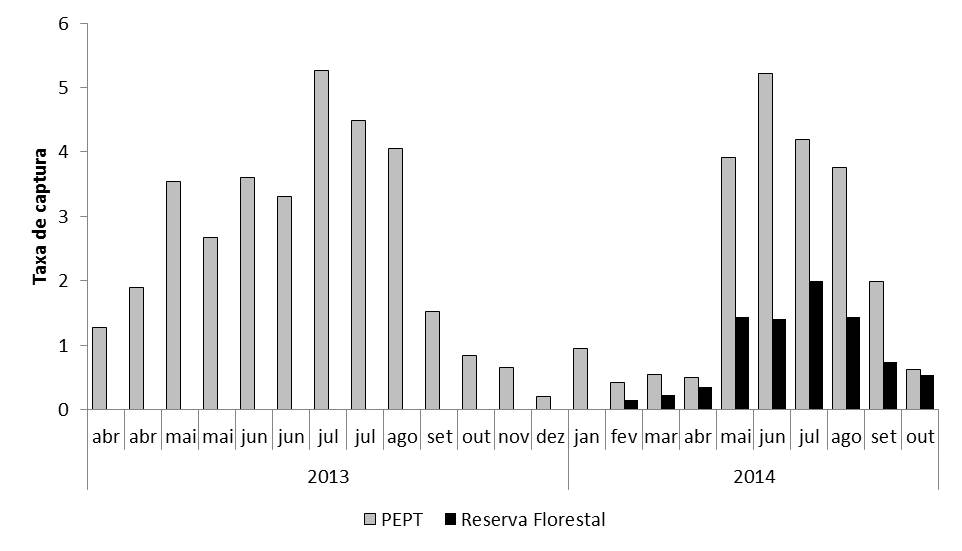
\includegraphics[width=0.75\textwidth]{figures/Imagem4/Imagem4.jpg}
  \caption{Distribuição temporal das taxas de captura (número de indivíduos/tempo de amostragem (min) * número de coletores) dos Ithomiini (Nymphalidae, Danainae) amostrados no Parque Esporte para Todos (PEPT) e na Reserva Florestal da Cidade Universitária Armando Salles Oliveira.}
  \label{fig:2.1.3} 
\end{figure}

\begin{figure}
  \centering
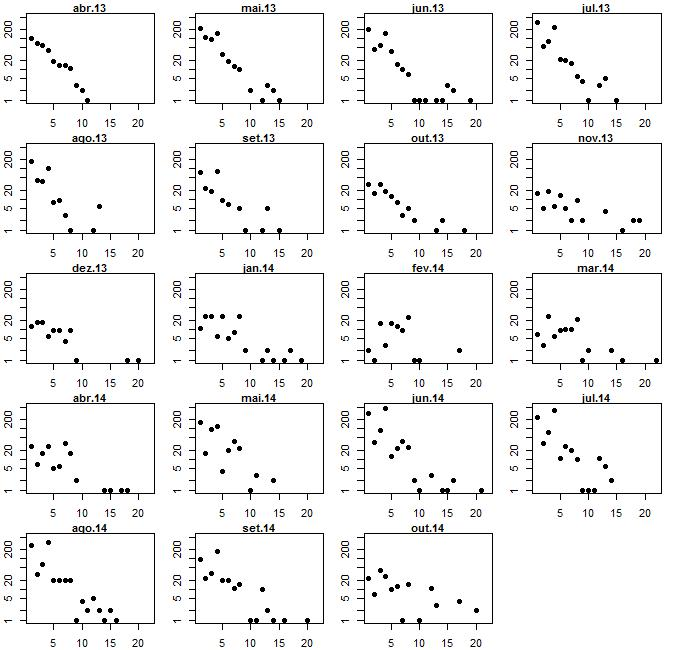
\includegraphics[width=0.75\textwidth]{figures/Imagem5/Imagem5.jpg}
  \caption{Distribuições de Abundância de Espécies (DAE) de Ithomiini obtidas em cada mês (abr/13 a out/14) no Parque Esporte Para Todos (PEPT). No eixo y está representado o número de indivíduos capturados e no eixo x estão representadas as 22 espécies registradas na área. A ordem das espécies (rank) é mantida constante ao longo dos meses.}
  \label{fig:2.1.4} 
\end{figure}

\begin{figure}
  \centering
  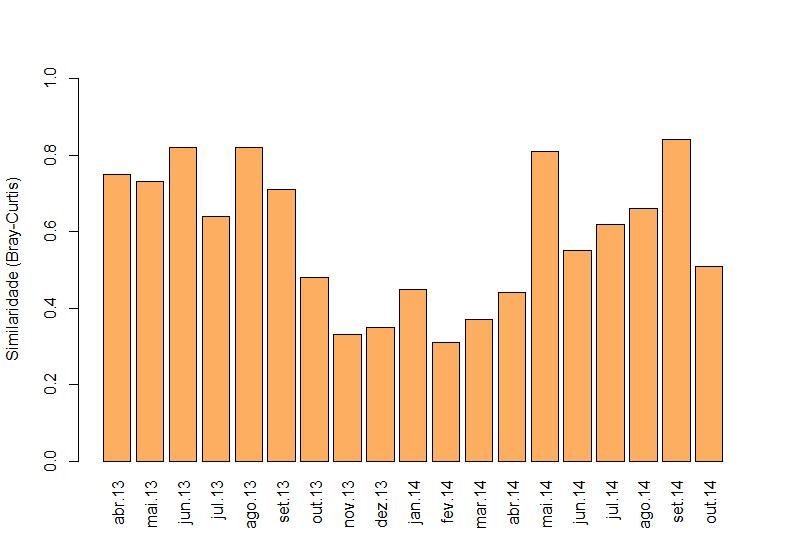
\includegraphics[width=0.75\textwidth]{figures/Imagem6/Imagem6.jpg}
  \caption{Similaridade de Bray-Curtis das amostras mensais de Ithomiini com o centróide da comunidade, o qual foi obtido calculando-se o número médio de indivíduos de cada espécie capturados por mês.}
  \label{fig:2.1.5} 
\end{figure}

\begin{figure}
  \centering
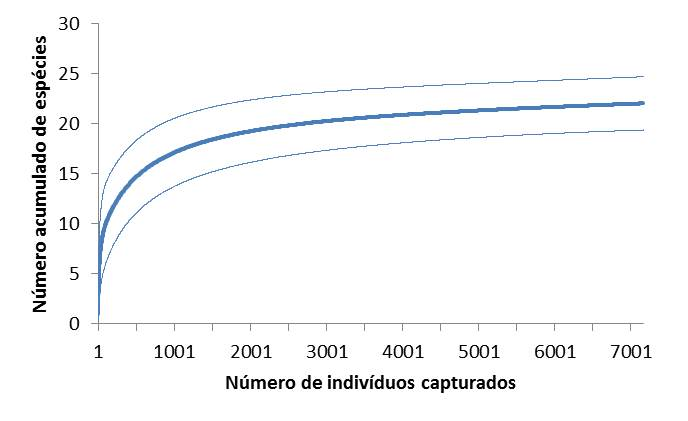
\includegraphics[width=0.75\textwidth]{figures/Imagem7/Imagem7.jpg}
  \caption{Curva espécies-tempo baseada em indivíduos obtida no Parque Esporte Para Todos entre abril/13 e outubro/14. Os dados foram aleatorizados 100 vezes e as linhas mais estreitas representam o intervalo de confiança (95 por cento). Nesta curva foram considerados indivíduos recapturados entre campanhas porém não dentro de uma campanha.}
  \label{fig:2.1.6} 
\end{figure}


\subsection{Aves: complexidade de habitats e diversidade} % Rodolpho
\label{sec:compl-de-habit} 

Até o momento foram realizadas duas das três saídas de campo previstas
para este subprojeto. A primeira viagem estava destinada a estudo piloto
e ajuste do delineamento amostral. Foi realizada entre 8 e 30 de
maio de 2014 e incluiu o reconhecimento das áreas, teste de dois
potenciais métodos amostrais (ponto fixo e transecto) 
e a definição dos sítios a serem amostrados nas próximas campanhas. 

A proposta inicial do projeto era utilizar o método de ponto de
fixo escuta, pois um dos objetivos do projeto, quantificação do uso dos
estratos vegetais pelas aves, depende da visualização direta dos
indivíduos. Nós acreditávamos que esta visualização poderia ser
facilitada se o observador estivesse parado em um mesmo local. No
entanto, o método de transecto também poderia ser mais vantajoso por
permitir a amostragem de uma área maior. 
 Após 12 dias de testes em 
pelo menos 5 áreas de cada fitofisionomia (campestre, cerrado, cerradão),
foram contabilizados 331 registros de 60 espécies usando o método de
ponto de escuta e 225 registros de 65 espécies utilizando o método de
transecto. No entanto, apenas 18\% de todos os registros feitos
utilizando o método de ponto de escuta foram visuais, contra 48\%
com  método de transecto. Esse resultado nos motivou a escolher o método de
transecto para a continuidade do trabalho.
Escolhemos então demarcados 32 sítios amostrais,
cada um composto de dois transectos de 200 m, distribuídos entre três
fitofisionomias distintas de Cerrado, a saber: campo sujo (12 sítios), campo
cerrado (10 sítios) e cerrado \textit{sensu stricto} (10 sítios). 
Estas fitofisionomias foram
escolhidas por representarem um gradiente de estrutura vegetacional,
que aumenta do campo sujo para o cerrado \textit{sensu stricto}, sendo
o campo cerrado a forma intermediária. Os sítios foram escolhidos entre
os de acesso viável no parque, distando no mínimo 1 km, buscando-se
evitar agregações de sítios de um só tipo de fisionomia. 
Nesta campanha também definimos os estratos vegetacionais para registro: 
\begin{description}
\item[herbáceo:] formado por capins e ervas de até 100cm altura, sem plantas com copa definida ou caule lignificado;
\item[arbustivo:] arbustos de até 100cm de altura: sem copa definida mas caule lignificado;
\item[arbórea baixa:] arvoretas e árvores de 100 a 300cm de altura, com copa definida;
\item[arbórea:] árvores acima de 300cm de altura. 
\end{description}


Na segunda campanha (25 de novembro e 17 dezembro de
2014) foi realizada a primeira etapa das amostragens nos 32 sítios. 
As amostragens foram realizadas nos períodos da manhã (entre 06:00 e
11:00) e tarde (entre 15:30 e 20:00), evitando os períodos com
incidência de chuva. Metade dos sítios foram visitados em
pelo menos duas ocasiões pela manhã, cada uma por um observador
diferente, o que irá possibilitar a análise da influência do
observador sobre o registro das espécies e também o
padrão de ocorrência das espécies por fitofisionomia. A outra metade
dos sítios foram visitados entre quatro e seis ocasiões pela manhã e
entre duas e quatro ocasiões à tarde, o que nos permitirá avaliar a
influência do período do dia na detecção das aves, assim como também
calcular a detecção para cada espécie e fisionomia. Em cada registro
foi considerada a presença da ave dentro ou fora de raio de 100m em torno do observador
e o tipo de registro (visual ou auditivo). Nos registros visuais, foi
medida a distância perpendicular das aves em relação ao
transecto, a qual será utilizada para avaliar o efeito da distância de
observação na detecção das aves, e também o estrato vegetacional em que o
indivíduo foi avistado. 

Contabilizados 1925 registros de aves de 141 espécies (Tab.~\ref{tab:aves1}).
O maior número de
registros foi obtido nos sítios de campo cerrado (653), seguido
por campo sujo (640) e cerrado \textit{sensu stricto}
(625). Entretanto, os
registros dentro do raio amostral de 100m foram mais numerosos na
fitofisionomia campo sujo (334), depois em campo cerrado (269) e por
último em cerrado \textit{sensu stricto} (214) (Fig.~\ref{fig:aves2}). 
Já para os
registros realizados fora do raio de 100m,
o cerrado \textit{sensu stricto} teve o maior número (414), 
seguido do campo cerrado (384) e
por último o campo sujo (306) (Fig.~\ref{fig:aves2}). 
Registramos mais espécies dentro do raio de 100m no
cerrado (67), seguido por cerrado \textit{sensu stricto} (64) e campo
sujo (60). Para fora do raio de 100m 
a fitofisionomia campo sujo apresentou um maior número de espécies (63), seguido por campo
cerrado (59) e cerrado \textit{sensu stricto} (26).
Estes resultados preliminares indicam que o número de registros de indivíduos e de espécies
diferem entre fitofisionomias. Além disso, 
os registros e espécies encontrados dentro e fora do raio de 100m
em torno dos pontos apresentam diferentes padrões. Este efeito da
distância pode ocorrer tanto por uma maior heterogeneidade de habitats
dentro e em torno de algumas fitofisionomias em relação à outras quanto por um
efeito da detectabilidade associado às características dos habitats,
já que o efeito positivo da vegetação sobre o número de espécies
poderia ser reduzido ou até mascarado por um efeito negativo da
vegetação sobre a detecção das espécies.

De fato, o efeito das fitofisionomias sobre a ocupação e também sobre
a detecção das espécies já se revela em uma análise preliminar
de ocorrência de três das cinco espécies mais registradas na
primeira campanha. A probabilidade de ocupação do  Tico-tico 
do campo  (\textit{Ammodramus humeralis}, 75 registros) 
diferiu entre três fitofisionomias amostradas
(Fig.~\ref{fig:aves5}), ao contrário de sua detecção. 
Como seu nome popular indica, esta espécie parece ocupar
preferencialmente áreas de campo sujo e campo cerrado, com menor
ocorrência em áreas com mais vegetação mais complexa. Já para o Chibum
(\textit{Elaenia chiriquensis}, 120 registros) e o Tesourão (\textit{Eupetomena
macroura}, 40), as estimativas indicam igual taxa de ocupação mas diferentes 
detectabilidade entre fitofisionomias 
(Fig.~\ref{fig:aves6}). O Chibum teve maior
probabilidade de detecção nas fisionomias campo cerrado e cerrado
\textit{sensu stricto}, pois nessas fisionomias a espécie costuma pousar nos poucos 
poleiros mais altos em busca de presas que passam em voo. Por sua vez,
\textit{E. macroura} teve maior probabilidade de detecção em cerrado
\textit{sensu stricto}, talvez simplesmente por
maior permanência e consequentemente detecção.
Dentro do raio de 100m em torno dos pontos o número de registros e 
espécies registradas  aumentou
do estrato herbáceo para o arbóreo (Fig.~\ref{fig:aves4}).  
Ainda não acumulamos 
dados o suficiente para fazer a análise de ocupação
por estrato, mas as diferenças podem pelo menos em parte dever-se 
à maior facilidade de detecção de indivíduos pousados
nos arbustos mais altos e árvores. 

Em resumo, as etapas previstas de delineamento e primeira amostragem
foram cumpridas. Transferimos a terceira campanha de amostragem do quarto para o
quinto trimestres de projeto, devido a atraso da estação chuvosa. 
A julgar pelos registros obtidos até o momento,
será possível estimar diferenças de ocupação das fitofisionomias
pelas espécies mais abundantes e também pela comunidade \citep{dorazio2005}.
Também é possível estimar as riquezas de espécies
em cada fisionomia, levando-se em conta eventuais diferenças de detecção \citep{dorazio2006}.
Há evidências de que a detecção também varia entre fisionomias,
e o delineamento foi planejado para estimá-las.
Dado que as fitofisionomias diferem marcadamente quanto à complexidade,
a confirmação de diferenças de ocupação e de riqueza ao testes
da hipótese de efeito da complexidade estrutural sobre a diversidade
de aves no cerrado. Uma segunda linha de evidência é a estimativa das
taxas de ocupação por estrato, o que depende de uma maior densidade de 
registros visuais na próxima campanha.

\begin{longtable}{>{\itshape}lrrrrrr}
\caption{Espécies de aves registradas na primeira campanha, com
    seu número de registros e de sítios em que houve registros, 
    para as fisionomias de Campo Cerrado (CC, 10 sítios), Campo sujo (CS, 12 sítios) 
    e Cerrado senso estrito (SS, 10 sítios).}\\
\toprule
& \multicolumn{3}{c}{N registros} & \multicolumn{3}{c}{N sítios} \\ 
\textbf{sp} & \textbf{CC} & \textbf{CS} & \textbf{SS} &  \textbf{CC} & \textbf{CS} & \textbf{SS} \\
\midrule
\endfirsthead
\multicolumn{7}{r}%
{\tablename\ \thetable\ -- \textit{Continuação}} \\
\toprule
& \multicolumn{3}{c}{N registros} & \multicolumn{3}{c}{N sítios} \\ 
\textbf{sp} & \textbf{CC} & \textbf{CS} & \textbf{SS} &  \textbf{CC} & \textbf{CS} & \textbf{SS} \\
\midrule
\endhead
\midrule \multicolumn{7}{r}{\textit{Continua}} \\
\endfoot
\bottomrule
\endlastfoot
    Alipiopsitta xanthops & 0 & 0 & 1 & 0 & 0 & 1 \\ 
    Amazilia fimbriata & 0 & 0 & 4 & 0 & 0 & 2 \\ 
    Amazona aestiva & 2 & 2 & 2 & 2 & 2 & 2 \\ 
    Ammodramus humeralis & 28 & 36 & 11 & 8 & 10 & 3 \\ 
    Aphantochroa cirrhochloris & 0 & 1 & 0 & 0 & 1 & 0 \\ 
    Ara ararauna & 0 & 1 & 0 & 0 & 1 & 0 \\ 
    Aratinga acuticaudata & 0 & 6 & 0 & 0 & 2 & 0 \\ 
    Aratinga aurea & 9 & 3 & 8 & 4 & 2 & 4 \\ 
    Athene cunicularia & 0 & 1 & 0 & 0 & 1 & 0 \\ 
    Barypthengus ruficapillus & 0 & 0 & 1 & 0 & 0 & 1 \\ 
    Basileuterus culicivorus & 0 & 1 & 0 & 0 & 1 & 0 \\ 
    Campephilus melanoleucus & 1 & 0 & 0 & 1 & 0 & 0 \\ 
    Camptostoma obsoletum & 7 & 4 & 7 & 4 & 3 & 4 \\ 
    Canthorchilus leucotis & 2 & 1 & 1 & 1 & 1 & 1 \\ 
    Caracara plancus & 1 & 0 & 0 & 1 & 0 & 0 \\ 
    Cariama cristata & 2 & 1 & 2 & 2 & 1 & 2 \\ 
    Chaetura meridionalis & 2 & 0 & 0 & 2 & 0 & 0 \\ 
    Chlorostilbon lucidus & 3 & 2 & 2 & 3 & 2 & 2 \\ 
    Chordeiles pusillus & 1 & 1 & 1 & 1 & 1 & 1 \\ 
    Cnemotriccus fuscatus & 0 & 0 & 1 & 0 & 0 & 1 \\ 
    Colaptes campestris & 1 & 1 & 1 & 1 & 1 & 1 \\ 
    Crypturellus parvirostris & 2 & 1 & 3 & 1 & 1 & 3 \\ 
    Crypturellus undulatus & 0 & 1 & 0 & 0 & 1 & 0 \\ 
    Culicivora caudacuta & 0 & 1 & 0 & 0 & 1 & 0 \\ 
    Cyanocorax chrysops & 2 & 0 & 0 & 2 & 0 & 0 \\ 
    Cyanocorax cristatelus & 4 & 3 & 7 & 2 & 2 & 4 \\ 
    Cyanocorax cyanopogon & 0 & 0 & 1 & 0 & 0 & 1 \\ 
    Cyclarhis gujanensis & 6 & 0 & 1 & 3 & 0 & 1 \\ 
    Cypsnagra hirundinacea & 4 & 0 & 3 & 4 & 0 & 1 \\ 
    Dryocopus lineatus & 0 & 0 & 1 & 0 & 0 & 1 \\ 
    Elaenia chiriquensis & 43 & 21 & 56 & 8 & 6 & 7 \\ 
    Elaenia cristata & 9 & 3 & 5 & 3 & 2 & 4 \\ 
    Elaenia flavogaster & 3 & 7 & 5 & 3 & 5 & 2 \\ 
    Emberezoides herbicola & 11 & 20 & 4 & 3 & 7 & 1 \\ 
    Eupetomena macroura & 7 & 7 & 26 & 4 & 6 & 9 \\ 
    Euphonia chlorotica & 1 & 1 & 2 & 1 & 1 & 1 \\ 
    Euscarthmus rufomarginatus & 0 & 7 & 0 & 0 & 1 & 0 \\ 
    Falco femoralis & 1 & 0 & 0 & 1 & 0 & 0 \\ 
    Falco sparverius & 0 & 0 & 1 & 0 & 0 & 1 \\ 
    Formicivora melanogaster & 0 & 0 & 4 & 0 & 0 & 4 \\ 
    Formicivora rufa & 5 & 1 & 8 & 2 & 1 & 3 \\ 
    Furnarius rufus & 2 & 0 & 0 & 1 & 0 & 0 \\ 
    Gnorimopsar chopi & 0 & 22 & 11 & 0 & 3 & 3 \\ 
    Heliactin bilopha & 9 & 5 & 4 & 5 & 3 & 4 \\ 
    Hemithraupis guira & 0 & 0 & 2 & 0 & 0 & 2 \\ 
    Hemitriccus margaritaceinventer & 3 & 0 & 0 & 3 & 0 & 0 \\ 
    Heterospizias meridionalis & 1 & 0 & 2 & 1 & 0 & 1 \\ 
    Knipolegus lophotes & 0 & 7 & 0 & 0 & 1 & 0 \\ 
    Legatus leucophaius & 0 & 0 & 1 & 0 & 0 & 1 \\ 
    Lepidocolaptes angustirostris & 3 & 1 & 15 & 2 & 1 & 7 \\ 
    Machetornis rixosus & 0 & 1 & 0 & 0 & 1 & 0 \\ 
    Megarynchus pitangua & 0 & 0 & 1 & 0 & 0 & 1 \\ 
    Megascops choliba & 0 & 0 & 1 & 0 & 0 & 1 \\ 
    Melanopareia torquata & 11 & 1 & 3 & 4 & 1 & 1 \\ 
    Milvago chimachima & 2 & 1 & 2 & 1 & 1 & 2 \\ 
    Mimus saturninus & 5 & 21 & 7 & 2 & 6 & 3 \\ 
    Myarchus swainsoni & 5 & 0 & 9 & 2 & 0 & 3 \\ 
    Myarchus tyrannulus & 0 & 3 & 0 & 0 & 1 & 0 \\ 
    Myophobus fasciatus & 0 & 4 & 0 & 0 & 4 & 0 \\ 
    Neothraupis fasciata & 8 & 0 & 1 & 4 & 0 & 1 \\ 
    Nystalus chacuru & 2 & 0 & 8 & 1 & 0 & 4 \\ 
    Pachyramphus polychopterus & 0 & 0 & 4 & 0 & 0 & 2 \\ 
    Parula pityaiumi & 0 & 0 & 1 & 0 & 0 & 1 \\ 
    Patagioenas cayennensis & 2 & 0 & 0 & 2 & 0 & 0 \\ 
    Patagioenas picazuro & 0 & 0 & 2 & 0 & 0 & 1 \\ 
    Phacellodomus rufifrons & 6 & 5 & 1 & 5 & 4 & 1 \\ 
    Phaethornis pretrei & 1 & 0 & 3 & 1 & 0 & 3 \\ 
    Picumnus albosquamatus & 1 & 0 & 0 & 1 & 0 & 0 \\ 
    Piranga flava & 0 & 0 & 2 & 0 & 0 & 2 \\ 
    Polioptila dumicola & 1 & 6 & 1 & 1 & 1 & 1 \\ 
    Porphyrospiza caerulescens & 0 & 1 & 0 & 0 & 1 & 0 \\ 
    Progne chalybea & 1 & 0 & 0 & 1 & 0 & 0 \\ 
    Psarocolius decumanus & 0 & 0 & 1 & 0 & 0 & 1 \\ 
    Ramphastos toco & 0 & 1 & 3 & 0 & 1 & 2 \\ 
    Ramphocellus carbo & 0 & 1 & 0 & 0 & 1 & 0 \\ 
    Rupornis magnirostris & 0 & 1 & 0 & 0 & 1 & 0 \\ 
    Rynchotus rufescens & 6 & 10 & 6 & 5 & 5 & 3 \\ 
    Saltator similis & 0 & 1 & 0 & 0 & 1 & 0 \\ 
    Saltatricula atricollis & 11 & 15 & 5 & 4 & 5 & 3 \\ 
    Scardafella squamata & 1 & 0 & 0 & 1 & 0 & 0 \\ 
    Schistochlamys melanopis & 3 & 0 & 0 & 1 & 0 & 0 \\ 
    Schistochlamys ruficapillus & 7 & 2 & 0 & 4 & 1 & 0 \\ 
    Schoeniophylax phryganophilus & 0 & 1 & 2 & 0 & 1 & 1 \\ 
    Sporophila angolensis & 0 & 1 & 0 & 0 & 1 & 0 \\ 
    Sporophila plumbea & 2 & 11 & 17 & 1 & 5 & 3 \\ 
    Stelgidopteryx ruficollis & 0 & 1 & 0 & 0 & 1 & 0 \\ 
    Suiriri islerorum & 4 & 17 & 5 & 2 & 2 & 2 \\ 
    Synalaxis albescens & 17 & 7 & 13 & 5 & 4 & 4 \\ 
    Synalaxis frontalis & 1 & 0 & 0 & 1 & 0 & 0 \\ 
    Tachornis squamata & 12 & 11 & 5 & 4 & 4 & 2 \\ 
    Tangara cayana & 0 & 0 & 1 & 0 & 0 & 1 \\ 
    Tangara palmarum & 0 & 10 & 5 & 0 & 4 & 2 \\ 
    Tangara sayaca & 0 & 0 & 1 & 0 & 0 & 1 \\ 
    Thamnophilus torquatus & 12 & 1 & 1 & 4 & 1 & 1 \\ 
    Troglodytes musculus & 11 & 8 & 23 & 4 & 5 & 8 \\ 
    Turdus leucomelas & 1 & 2 & 2 & 1 & 2 & 2 \\ 
    Tyrannus albogularis & 3 & 5 & 4 & 2 & 3 & 2 \\ 
    Volatinia jacarina & 0 & 1 & 0 & 0 & 1 & 0 \\ 
    Xolmis cinereus & 0 & 4 & 0 & 0 & 4 & 0 \\ 
    Xolmis velatus & 0 & 3 & 2 & 0 & 1 & 1 \\ 
    Zonotrichia capensis & 30 & 22 & 37 & 7 & 8 & 8 \\ 
  \label{tab:aves1}
\end{longtable}


\begin{figure}
  \centering
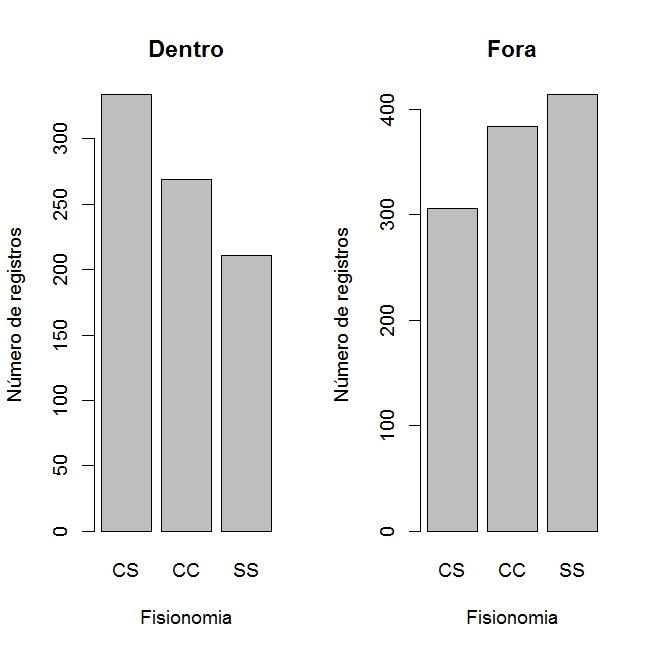
\includegraphics[width=0.5\textwidth]{figures/reg_fito/reg_fito.jpg}
  \caption{Número de registros de aves realizados em cada uma das fitofisionomias amostradas, considerando os rgistros feitos dentro do raio amostral de 100m e fora deste raio amostral. Legenda: CS- campo sujo; CC -  campo cerrado; SS- cerrado \textit{sensu stricto}. Note que o comprimento do eixo y é diferente nos dois gráficos.}
  \label{fig:aves2} 
\end{figure}

\begin{figure}
  \centering
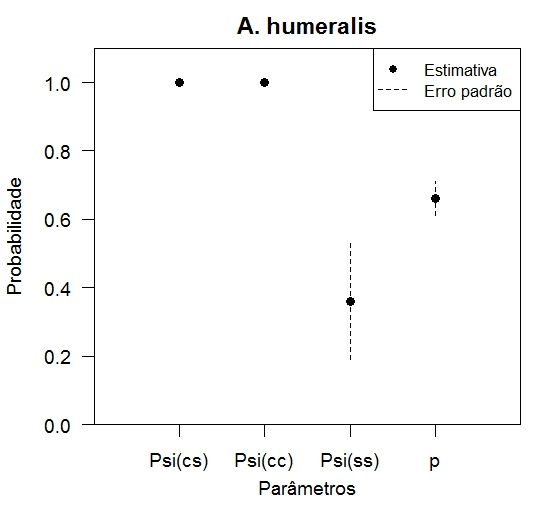
\includegraphics[width=0.5\textwidth]{figures/ocupacao/ocupacao.jpg}
  \caption{Valores de parâmetros estimados e erro padrão das estimativas de ocupação e detecção da espécie de ave \textit{Ammodramus humeralis}, para três fitofisionomias de cerrado. Legenda: Psi(cs)- probabilidade de ocupação em campo sujo; Psi(cc)- probabilidade de ocupação em campo cerrado; Psi(cs)- probabilidade de ocupação em cerrado \textit{sensu stricto}; p- probabilidade de detecção.}
  \label{fig:aves5} 
\end{figure}

\begin{figure}
  \centering
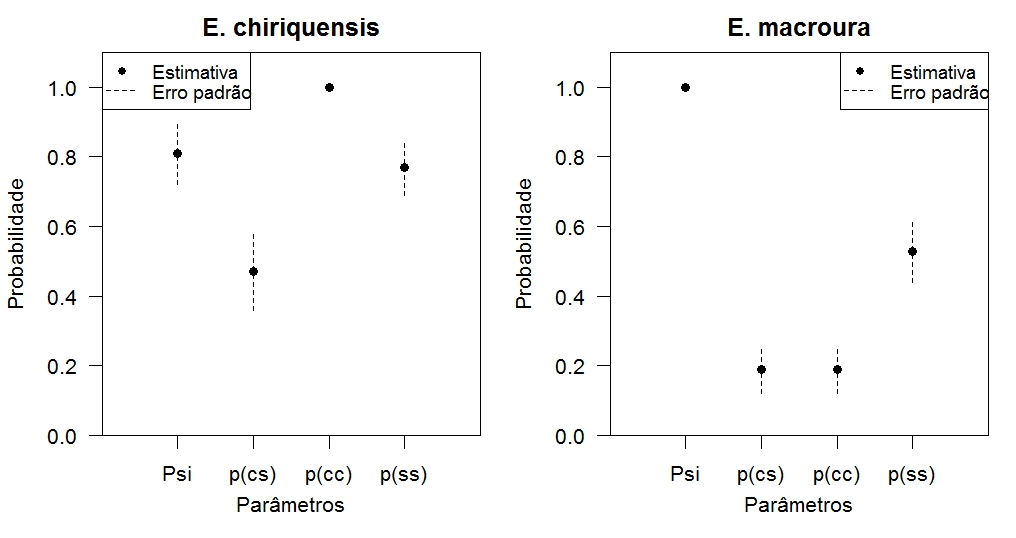
\includegraphics[width=0.75\textwidth]{figures/deteccao/deteccao.jpg}
  \caption{Valores de parâmetros estimados e erro padrão das estimativas de ocupação e detecção das espécies de aves \textit{Elaenia chiriquensis} e \textit{Eupetomena macroura}, para três fitofisionomias de cerrado. Legenda: Psi- probabilidade de ocupação; p(cs)- probabilidade de detecção em campo sujo; p(cc)- probabilidade de detecção em campo cerrado; probablilidade de detecção em cerrado \textit{sensu stricto}.}
  \label{fig:aves6} 
\end{figure}

\begin{figure}
  \centering
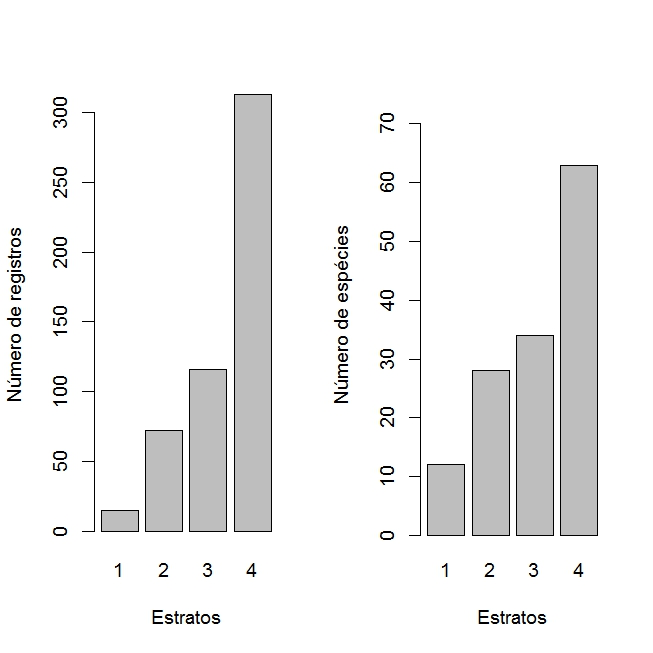
\includegraphics[width=0.5\textwidth]{figures/dados_strata/dados_strata.jpg}
  \caption{Número de registros e de espécies observados em cada um dos estratos vegetacionais definidos, considerando apenas os registros feitos dentro do raio amostral de 100m. 
A definição dos estratos vegetacionais encontra-se no corpo do texto. Note que a escala do eixo y é diferente nos dois gráficos.}
\label{fig:aves4} 
\end{figure}

\subsection{Baleias: dinâmica populacional e flutuações climáticas} % Leo
\label{sec:dinam-popul-de}
%% Além dos resultados e análise já realizados, indicar rede de
%% colaborações estabelecidas e como se articulam com o projeto.
Entre julho e novembro de 2014 foram realizadas campanhas marítimas
embarcadas para contagem e foto-identificação de baleias-jubarte no
Banco dos Abrolhos (Fig.~\ref{fig:baleia1}). 
Com esta amostragem de 2014, completamos 25
anos de série temporal de dados disponíveis para as análises de taxas
demográficas e dinâmica populacional dessa espécie em sua área
reprodutiva no Brasil.


Foram realizadas dez campanhas de campo, totalizando 28 dias de
amostragem de 1.150 milhas náuticas percorridas
(Tab.~\ref{tab:baleia1}). Durante a temporada reprodutiva de 2014,
295 grupos de baleias-jubarte foram aproximados pela embarcação,
resultando em um total de 273 baleias-jubarte identificadas através de
marcas naturais na parte ventral da nadadeira caudal (Fig.~\ref{fig:baleia2}). 
Uma análise preliminar revelou pelo menos nove reavistamentos de
baleias identificadas em anos anteriores, mas esse número deve
aumentar substancialmente após a realização da comparação com
a base de fotos dos censos anteriores,
que está em andamento. Amostras de pele para extração de DNA
micro-satélites, que também permite a identificação individual, foram
coletadas para 91 indivíduos. As amostras de tecido para análises
genéticas foram enviadas para o Laboratório de Biologia
Genômica e Molecular da Pontifícia Universidade Católica do Rio Grande
do Sul, e irão compor o catálogo de identificação genética de baleias.

\begin{table}
\centering
\caption{Censo fotográfico realizado durante a temporada reprodutiva da baleia-jubarte no Banco dos Abrolhos em 2014:
Esforço amostral em número de dias embarcados e distância percorridas (milhas náuticas), e número de grupos avistados,
por campanha de amostragem.}
\begin{tabular}{cccrc}
\toprule  
    \textbf{Campanha} & \textbf{Datas} & \textbf{N Dias} & \textbf{Dist} & \textbf{N Grupos} \\
\midrule
    01 & 02 a 04 de agosto & 3 & 129,0 & 38 \\
    02 & 21 a 23 de agosto & 3 & 126,6 & 39 \\
    03 & 27 a 29 de agosto & 3 & 115,3 & 29 \\
    04 & 11 a 13 de agosto & 3 & 122,1 & 41 \\
    05 & 24 a 26 de setembro & 3 & 138,1 & 34 \\
    06 & 08 a 10 de outubro & 3 & 109,2 & 31 \\
    07 & 24 a 26 de outubro & 3 & 93,1 & 28 \\
    08 & 01 a 04 de novembro & 4 & 209,7 & 29 \\
    09 & 07 e 08 de novembro & 2 & 66,5 & 18 \\
    10 & 12 de novembro & 1 & 39,2 & 08 \\
    \textbf{TOTAL} & & \textbf{28} & \textbf{1.149,9} & \textbf{295} \\
\bottomrule
  \end{tabular}
  \label{tab:baleia1}
\end{table}

A primeira etapa das análises é a estimativa do potencial biológico da população.
Para isso combinamos uma série temporal de 11 anos de levantamentos aéreos e 22
anos de dados de identificação individual das baleias-jubarte 
para estimar as taxas de crescimento dessa população,com métodos que consideram a
detecção imperfeita. Para os levantamentos aéreos
foram construídas funções de detecção anuais com os dados de
amostragem de distâncias perpendiculares dos grupos com relação às
linhas de transecção. Essas funções de detecção descrevem como a
probabilidade de detecção de grupos de baleias decresce conforme a
distância da linha. Calcula-se então a densidade de baleias
considerando a probabilidade de detecção em uma faixa determinada de
distância da linha de transecção, resultando em estimativas mais
robustas de abundância. Os dados de foto-identificação foram
analisados utilizados modelos de marcação-recaptura, que permitem o
cálculo de probabilidades de captura para os indivíduos marcados da
população, resultando em estimativas de sobrevivência e taxa de
crescimento mais robustas. Essas análises estão descritas no
manuscrito que se encontra anexo a este relatório, que mostra que
as taxas de crescimento no período são altas e possivelmente estão próximas
das taxas intrínsecas da espécie. O manuscrito está
em fase final de revisão pelos autores e será submetido durante a
vigência do auxílio.

Este componente, portanto, tem já uma série histórica de dados adequada
para responder às questões propostas. As próximas etapas, conforme previsto,
são completar as identificações das fotos dos últimos 3 anos, que está em andamento
em parceria coma equipe do Instituto Baleia Jubarte. 
Também realizaremos a  coleta das informações climáticas 
que fornecerão as covariáveis para os modelos. Para isso estabelecemos uma 
parceria com Prof. Dra. Ilana Wainer, do Instituto Oceanográfico da USP.


\begin{figure}
  \centering
  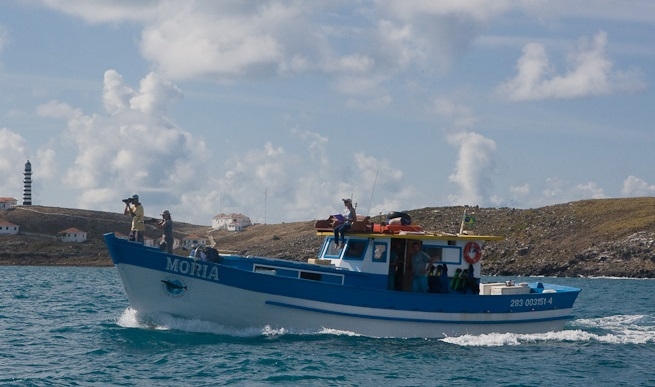
\includegraphics[width=0.75\textwidth]{figures/crop_Moria2/crop_Moria2.jpg}
  \caption{Embarcação \textit{Moriá}, utilizada para a amostragem de baleias-jubarte no Banco dos Abrolhos em 2014.
    É um \textit{trawler} com casco de madeira de ca. 15 metros de comprimento.}
  \label{fig:baleia1} 
\end{figure}


\begin{figure}
  \centering
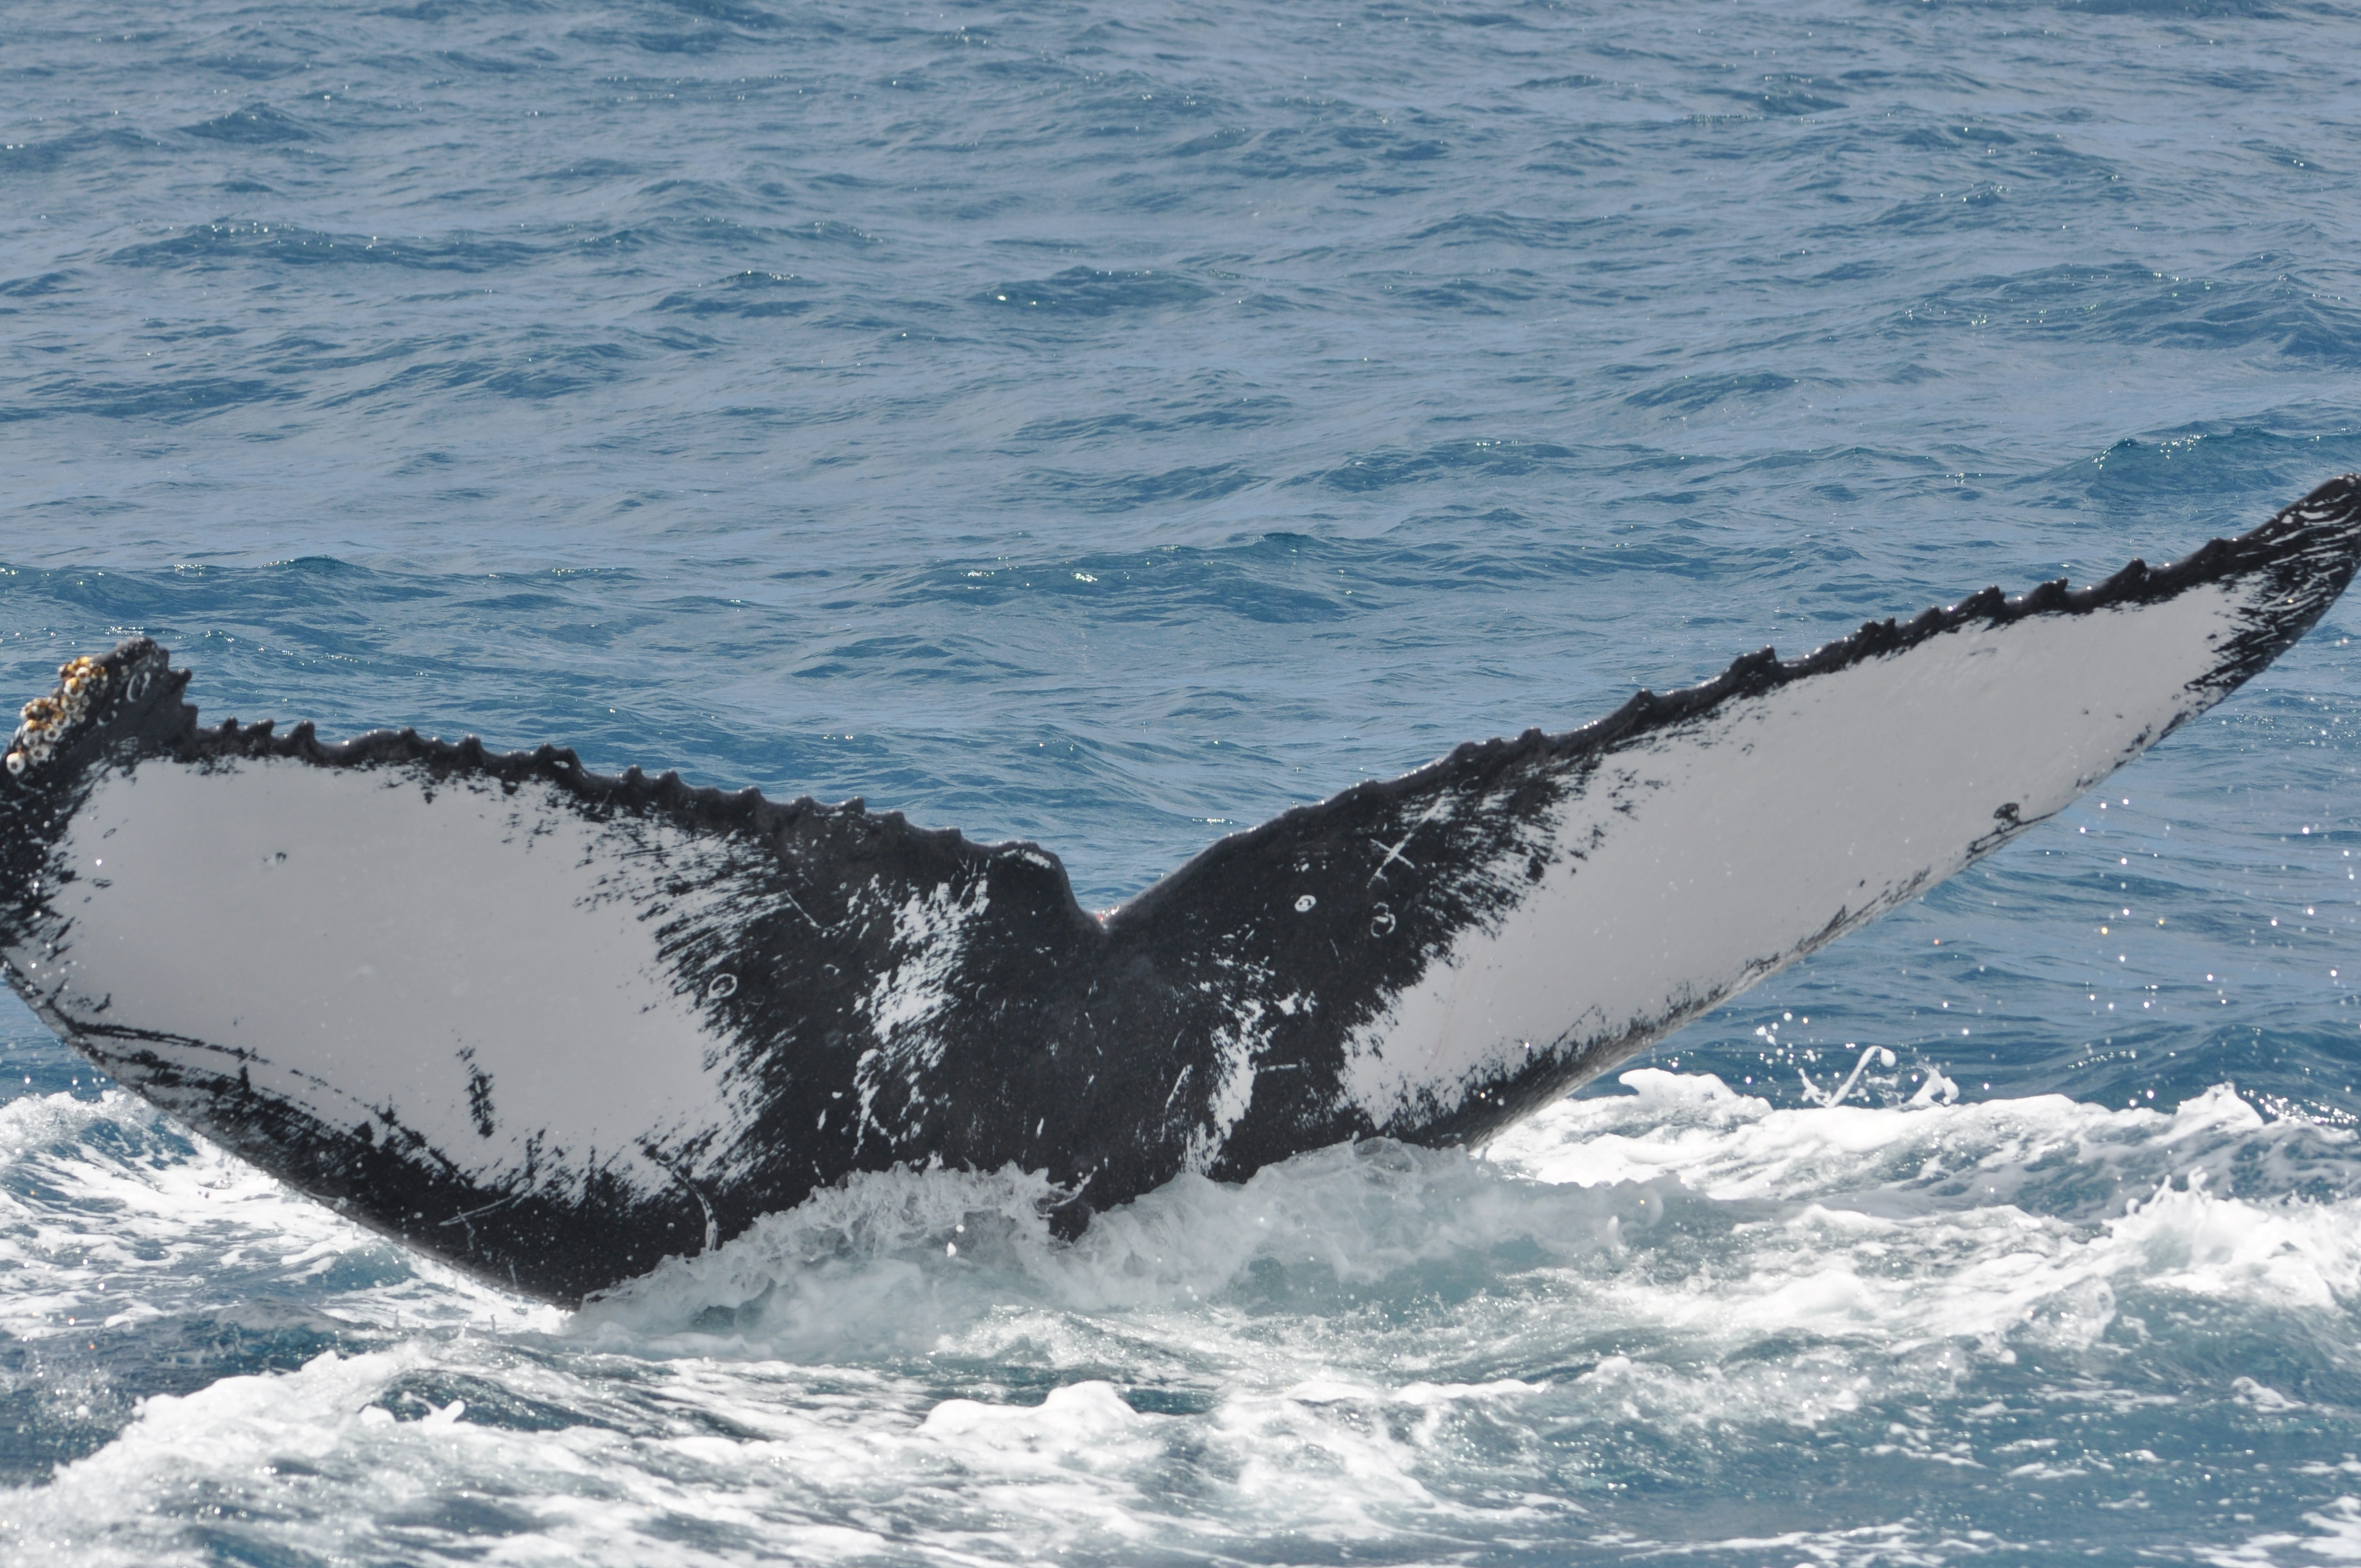
\includegraphics[width=0.75\textwidth]{figures/DSC_0393/DSC_0393.JPG}
  \caption{Parte ventral da nadadeira caudal de uma baleia-jubarte foto-identificada  no Banco dos Abrolhos em 2014.}
\label{fig:baleia2} 
\end{figure}


\section{Conclusões} %PI
Como previsto no cronograma original, realizamos boa parte das amostragens dos censos de borboletas e aves,
o que foi precedido por pilotos e planejamento do delineamento amostral. 
A base de dados de baleias foi ampliada com mais uma
amostragem, mantido delineamento já definido. 
Além disso, iniciamos análises parciais, também como previsto.
A única alteração em relação ao cronograma original 
é a realização do segundo censo de aves no quinto trimestre do projeto, e não no quarto. 
A julgar pelos resultados obtidos até o momento, teremos três excelentes bases de dados para realizar
as estimativas com e sem detecção imperfeita.

\section{Apoio institucional} %PI
Recebi todo o apoio institucional necessário, que foi detalhado no formulário de infraestrutura institucional, 
encaminhado com o termo de outorga. 

\section{Aplicação da RT e benefícios complementares} %PI
Neste período usei a reserva técnica para adquirir dois notebooks (R\$5467,96)
com um suporte e um monitor adicional de vídeo (R\$600,00).
O equipamento é usado pela equipe no processamento e análise dos dados.
Também adquiri cerca de R\$1500,00 em material de consumo para atividades de campo
(e.g. material de escritório, primeiros socorros, equipamento de segurança).

\section{Produção no período} 
Conforme as instruções da FAPESP, incluo esta seção. 
Cópia do manuscrito foi anexada ao sistema SAGe, na aba ``Outros documentos''.

\subsection{Manuscritos a submeter}
\label{sec:manuscritos-submeter}
Wedekin, L.L., Engel, M.H., Neves, M.C., Andriolo, Marcondes, M.C.C., Prado, P.I., Kinas, P.G., Zerbini, A.N., 
Simões-Lopes, P.C. Running fast in the slow lane: rapid population growth of the humpback whale after whaling. A ser submetido a \emph{Journal of Animal Ecology}

\subsection{Outros produtos}
\label{sec:outros-produtos}

Conforme previsto em nossos objetivos de disseminação de conhecimento, 
criamos uma disciplina no Programa de Pós-graduação em Ecologia da USP de introdução
a modelos populacionais com detecção imperfeita. O primeiro oferecimento foi em otubro de 2013,
com 14 alunos matriculados. O próximo oferecimento será em março de 2015. 
Desenvolvemos um sítio de redação colaborativa (wiki) com os roteiros e exercícios da disciplina: 
\url{http://ecologia.ib.usp.br/bie5703}. A disciplina é coordenada por Leonardo Wedekin e Paulo Inácio Prado,
e conta com a participação de toda a equipe na monitoria e apresentação de palestras.

\bibliographystyle{ecol_let}
\bibliography{biblio}

\end{document}
